\documentclass[frenchb]{article}
\usepackage[T1]{fontenc}
\usepackage[utf8]{inputenc}
\usepackage[francais]{babel}
\usepackage{fancyhdr}
\usepackage{float}
\usepackage{lastpage}
%\usepackage{fancyvrb}
\usepackage{graphicx}
\usepackage{hyperref}
\usepackage{caption}
\usepackage{subcaption}
\usepackage{microtype}
\usepackage{amsmath}
\usepackage{amssymb}

\pagestyle{fancy}
\rhead{Etat de l'art}
\cfoot{Mathias BRULATOUT}
\rfoot{\thepage}

\renewcommand{\footrulewidth}{0.5pt}

\begin{document}
\topmargin = 0.mm
\headheight = 12.1638pt
\evensidemargin = 10.mm


\tableofcontents
\clearpage

\section*{Objectif}
Pour un réseau ad-hoc comportant une multitude de connections TCP, avec un taux de perte et une gigue du RTT pouvant être élevés, analyser les différentes solutions possible pour les différentes configurations, permettant d'optimiser le débit utile, tout en limitant les changements de la pile protocolaire en garantissant au maximum les principales fonctionnalités de TCP à savoir :
\begin{itemize}
\item contrôle de flux.
\item contrôle de congestion.
\item fiabilité.
\item fairness et friendliness.
\end{itemize}

\section*{Introduction}
TCP a été conçu pour fonctionner sur des réseaux câblés, où les pertes de paquets ne sont dues qu'à des problèmes de congestion du réseau. TCP considère ainsi toute perte de paquet comme signe de congestion. La congestion est traitée de manière plutôt aggressive, puisque la fenêtre de congestion voit sa taille divisée par deux (donc débit divisé par deux) suite à une perte de paquet, et ne s'agrandit que de peu (un Maximum Segment Size) de façon constante(tous les Round Trip Time). C'est le principe de l'AIMD (Additive Increase, Multiplicative Decrease). Cela permet de conserver un équilibre entre les différents flux.

Dans un canal avec pertes, TCP détectera donc beaucoup de congestion, alors que ces erreurs sont bien souvent la conséquence d'interférences ou d'atténuations, et l'utilisation du canal sera loin d'être optimal. Des alternatives à celà permettent de contourner légèrement le problème. On peut par exemple utiliser un flag de TCP ECN (Explicit Congestion Notification), mais il faudrait changer toute la pile protocolaire des équipements réseaux ainsi que désactiver le backoff automatique en cas de perte si le flag ECN n'est pas placé.

Malgré tout, TCP reste fiable, et conserve toutes ses propriétés, mais sous-utilise grandement le canal dès que le taux d'erreur dépasse les 5\%. Il s'agit donc ici d'étudier différentes solutions permettant de garantir les diverses fonctionnalités de TCP tout en atteignant des performances proches de la capacité maximale du lien pour des taux de pertes de paquets élevés et potentiellement variables.

Ce document vise a pour but de décrire l'état de l'art dans le domaine de la fiabilisation sur des réseaux sans fils, en partant des techniques les plus simples, aux plus abouties mixant différents mécanismes.


\clearpage

\section{Quelques techniques}
Cette partie présente différentes solutions pour réparer les erreurs sur un canal avec pertes. Deux principaux mécanismes de récupération d'erreurs sont présentés : 
\begin{description}
\item [Réactifs :]  basés sur des retransmissions présenté section \ref{ARQ}.
\item [Proactifs :] basés sur du codage présenté section \ref{FEC}.
\end{description}
\subsection{ARQ : Automatic Repeat reQuest}
\label{ARQ}
C'est une méthode de contrôle d'erreur. En utilisant des acquittements, et des time-out, il s'agit de renvoyer des paquets non-acquittés au bout d'un certain temps.
Seul, ce mécanisme doit être de préférence utilisé au niveau 2 du modèle OSI, comme l'a montré \cite{llfeqarq}, qui permet de savoir plutôt rapidement comment le paquet a été perdu. Cela force une gestion \textbf{hop-by-hop} du paquet, s'avérant utile si des liens avec et sans pertes sont présents sur le chemin.
Trois techniques d'ARQ sont utilisées, à savoir :
\begin{description}
\item[Stop and Wait :] Le plus simple. Ici, on se contente d'envoyer une paquet et d'attendre son acquittement. S'il n'est pas reçu par l'envoyeur (le paquet ou son acquittement ont été perdus) au bout d'un certain temps, il est automatiquement renvoyé. Voir Figure \ref{fig:sub1}.
\item[Go Back N :] Même principe que le Stop and Wait avec la gestion d'une fenêtre d'emission. On envoie tous les paquets de la fenêtre d'emission de taille spécifiée. Si l'un deux n'est pas acquitté, on le renvoie lui ainsi que tous ceux d'après (qu'ils soient bien reçus la première fois ou pas). TCP utilise ce mécanisme particulièrement inneficace. Voir Figure \ref{fig:sub2}.
\item[Selective Repeat :] Plus flexible que le Go Back N, le receveur accepte les paquets même s'il a rencontré une erreur sur un paquet précédent. A l'aide d'un NACK il informe l'expéditeur de la non-reception d'un paquet, qui sera alors retransmit une fois que tout ce qui se trovue dans la fenêtre d'emission aura été envoyé. Voir Figure \ref{fig:sub3}.
\end{description}

\begin{figure}[H]
\centering
\begin{subfigure}{.5\textwidth}
  \centering
  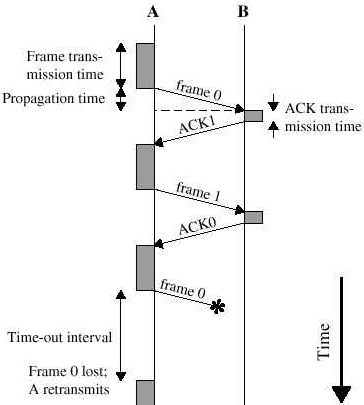
\includegraphics[width=\linewidth]{img/arq1.png}
  \caption{Stop and Wait.}
  \label{fig:sub1}         
\end{subfigure}%
\begin{subfigure}{.5\textwidth}
  \centering
  \vspace*{2.7cm}
  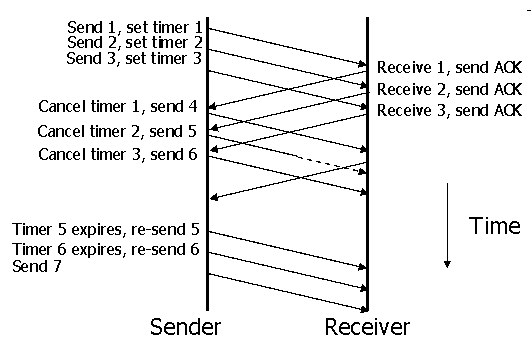
\includegraphics[width=\linewidth]{img/arq2.png}
  \caption{Go Back N.}
  \label{fig:sub2}
\end{subfigure}
\begin{subfigure}{\textwidth}
  \centering
  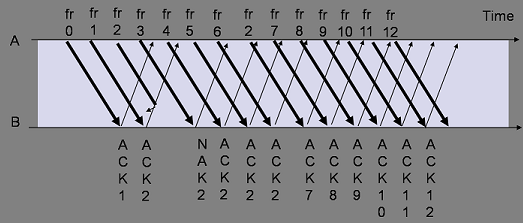
\includegraphics[scale=0.6]{img/arq3.png}
  \caption{Selective Repeat.}
  \label{fig:sub3}
\end{subfigure}
\caption{Les trois différents types d'ARQ.}
\label{fig:test}
\end{figure}

L'ARQ dans toutes ses formes permet de garantir la fiabilité. Cependant, il est nécessaire d'attendre au moins un RTT en cas d'erreur pour obtenir le paquet attendu (le retour de l'ACK puis le renvoi du paquet). Dans des applications en temps-réel où le délai est crucial ou sur des communications avec un RTT élevé telle que des communications satellites, il n'est pas raisonable de se baser uniquement sur un tel mécanisme de retransmission.
De plus, bien que fiabilisant les échanges, l'utilisation de l'ARQ n'améliore pas forcément l'utilisation de la bande passante notamment pour du multicast tel que le présente \cite{arqfornc}. L'ARQ n'est pas non plus tolérant aux délais, et est très sensible à la perte d'acquittements.

Une alternative est d'introduire de la redondance  de préférence avec du codage pour améliorer l'utilisation du lien.
 
\subsection{FEC : Forward Error Correction}
\label{FEC}
FEC ou code correcteur est une technique de codage basée sur la redondance. L'idée est de ne pas renvoyer de paquet en cas d'erreur, et donc d'introduire une redondance au moins égale au taux de perte des paquets, afin que le destinataire puisse avoir toutes les informations nécessaires après un envoi unique. Aucun acquittement n'est nécessaire, et donc un canal unidirectionnel suffit à faire du FEC, ce qui est assez pratique pour du broadcast par exemple.
Pour faire circuler $k$ paquets, on en envoit $n$ codés, avec $n>k$ et $n-k$ le facteur de redondance. Le récepteur doit recevoir au moins $k$ paquets codés pour retrouver les paquets originaux. S'il en reçoit moins, il ne pourra rien recoder. Il faut donc adapter avec précaution le taux de redondance pour optimiser le canan ltout en s'assurant de tarnsmettre assez d'informations.

Le théorème de Shannon a une place important en FEC puisquil définit la quantité maximale d'information utile pouvant passer par un canal ayant un certain taux de perte. En augmentant la complexité de l'encodage et du décodage, on peut approcher cette limite théorique. Il faut donc trouver un compromis entre ces deux paramètres.

Les codes par blocs sont souvent utilisés et il en existe un grand nombre :
\begin{itemize}
\item Code de répétition
\item Code de Reed-Salomon
\item Contrôle de parité de faible densité (LDPC)
\item Code Turbo
\item Code Raptor
\end{itemize}


Le problème du FEC, cité plus haut, est principalement le temps de codage et de décodage. Pour une implémentation au dessous du niveau 4, des temps trop longs dus à un codage trop complexe peuvent causer des timeout aux protocoles des couches supérieures. De plus, les codages doivent être fait de bout en bout, puisque la plupart de ces codages ne peuvent pas êtres composés. Le Random Linear Network Coding vu section \ref{RLNC} permet de composer le codage à plusieurs endroits du réseau tout en gardant sa cohérence.


Le tableau \ref{table:fecarq}, de \cite{feqarqtable} résume les différents aspects du FEC et de l'ARQ. \\ 
\begin{table}[H]
  \centering
  \begin{tabular}{|c|c|c|}
    \hline
    & \textbf{FEC} & \textbf{ARQ} \\
    \hline
    Fiabilité & Non & Oui\\
    \hline
    Améliore le transport & Oui & Non\\
    \hline
    Transmission en temps-réel & Oui & Non\\
    \hline
    Tolère les délais & Oui & Non\\
    \hline
    Tolère la perte d'ACK & N/A & Non\\
    \hline
  \end{tabular}
  \caption{Fonctionnalités de FEC \& ARQ}
  \label{table:fecarq}
\end{table}

Globalement, un système demandant une faible latence, ou n'ayant pas de mémoire ne pourra pas utiliser d'ARQ et donc devra utiliser du FEC. L'utilisation d'ARQ nécessite un canal de retour.

\subsection{H-ARQ : Hybrid ARQ}
Une solution efficace est de mixer FEC et ARQ, notamment appelé H-ARQ (pour Hybrid-ARQ), combinant du FEC à de l'ARQ quand les pertes sont trop importantes pour être contrées par la redondance prévue par le FEC.
Il en existe deux formes :
\begin{description}
\item[Type 1 :] Tous les messages composants des blocs sont envoyés avec FEC. Si le recepteur n'a pas assez d'information pour reconstruire un bloc, il demande la retransmission du bloc entier via l'ARQ.
\item[Type 2 :] Les messages sont envoyés en clair. Si une erreur est détectée, le recepteur utilise l'ARQ pour demander du code correcteur et éventuellement quelques bits de parités en plus.
\end{description}
L'H-ARQ, surtout de type 2, obtient de meilleures performances que l'ARQ et que le FEC. Ils sont bien souvent utilisés par des technologies comme Wimax mais peu répandues sur les couches supérieures


\subsection{Divers changements à TCP}
\subsubsection{TCP HACK : TCP with HeAder CheKsum}
TCP HACK, introduit par \cite{tcphack}, repose sur l'ajout d'une option au header TCP. Négociée lors du hanshake, cette option permet d'effectuer un checksum du header. Lors d'une erreur de checksum sur tout le paquet TCP, le checksum du header est aussi vérifié. S'il est cohérent, un ACK spécial est envoyé, ce qui permet de différencier une perte d'une congestion. L'expéditeur doit donc retransmettre le paquet. Cette solution semble plus efficace une fois couplée avec un mécanisme de SACK (Selective ACK). Le mécanisme de retransmission rend l'implémentation toujours dépendante du RTT et implique des changements de l'implémentation côté emetteur et récepteur.


\subsubsection{SpecTCP : Speculative TCP}
L'idée ici est de ne pas diminuer la fenêtre de congestion de TCP lors d'une perte indiquée par un timeout (associée à de la congestion). Le flag ECN (Explicit Congestion Notification) est utilisé. Tout le réseau doit être capable d'utiliser ce flag et une politique de gestion de queue RED (Random Early Discard), qui une fois couplée avec l'ECN permet de diminuer grandement la probabilité d'obtenir une congestion. Cette solution implique de gros changements sur tous les équipements réseaux traversés.

\subsubsection{LT-TCP : Loss Tolerant}
\cite{lt-tcp} présente LT-TCP, implémenté comme une couche fine entre TCP et IP. Utilisant seulement l'ECN comme signe de congestion, il fiabilise la tarnsmission via deux types de FEC :
\begin{itemize}
\item Proactive FEC : Estimation du taux d'erreur et envoi de FEC avec de la redondance adaptative.
\item Reactive FEC : Après la réception d'un SACK, faisant office d'ARQ (suite à plus d'erreurs que prévus lors de la phase proactive), un FEC est envoyé.
\end{itemize}
LT-TCP adapte aussi le MSS pour garder une granularité dans la fenêtre de congestion pour s'adapter au taux de redondance.
EN utilisant de nombreux mécanismes (FEC, ARQ, SACK, ajustement du MSS), LT-TCP parvient à de meilleurs résultats que du FEC ou H-ARQ de couche 2 et que TCP avec SACK.
Cependant cette version du protocole nécessite l'emploi du flag ECN sur tout le réseau, ce qui reste contraignant. Si le taux d'erreur dépasse les 40\%, LT-TCP voit ses performances chuter, suite à de trop nombreux timeout de la couche transport, que le FEC adaptatif ne peut contrer.


\subsection{RLNC : Random Linear Network Coding}
\label{RLNC}
L'idée de ce codage est de transmettre des combinaisons linéaires de paquets. Il suffit que le récepteur obtienne $n$ combinaisons linéiares indépendantes de $n$ paquets pour avoir assez d'informations et décoder les paquets.
Soit la matrice de coefficient $C_{n,n} =
 \begin{pmatrix}
  c_{1,1} & c_{1,2} & \cdots & c_{1,n} \\
  c_{2,1} & c_{2,2} & \cdots & c_{2,n} \\
  \vdots  & \vdots  & \ddots & \vdots  \\
  c_{n,1} & c_{n,2} & \cdots & c_{n,n}
 \end{pmatrix}$

ett un vecteur de paquets $X_n = 
\begin{pmatrix}
x_1\\
x_2\\
\vdots\\
x_n
\end{pmatrix}$\\
Les messages codés seront de la forme $$Y_n =
\begin{pmatrix}
y_1\\
y_2\\
\vdots\\
y_n
\end{pmatrix} =
\begin{pmatrix}
  c_{1,1} & c_{1,2} & \cdots & c_{1,p} \\
  c_{2,1} & c_{2,2} & \cdots & c_{2,p} \\
  \vdots  & \vdots  & \ddots & \vdots  \\
  c_{n,1} & c_{n,2} & \cdots & c_{n,p}
\end{pmatrix} 
\begin{pmatrix}
x_1\\
x_2\\
\vdots\\
x_n
\end{pmatrix}$$

avec $$y_i = \sum_{k=1}^{n} c_{i,k}x_k$$

Pour retrouver les messages encodés, il suffit de calculer la matrice inverse $C_{n,n}^{-1}$ de $C_{n,n}$ et d'en faire le produit avec les messages codés.
Pour éviter d'envoyer des combinaisons inutiles (linéairement dépendantes), et donc réduire le débit utile, les coefficients $c_{i,j}$ doivent être choisis dans un corps assez grand. \cite{practicalnetwork} étudie la taille du corps dans lequel les coefficients sont choisis démontre que 8 bits suffisent pour encoder les différents coefficients. En effet, dans le corps $\mathbb{F}(2^8)$, la probabilité d'obtenir deux combinaisons linéaires dépendantes est très faible. L'utilisation du corps $\mathbb{F}(2^{16})$ double la taille des coefficients et ne permet pas d'obtenir un gain de performance intéressant. Le livre sur la cryptographie \cite{java} présente l'optimisation des opérations dans le corps $\mathbb{F}(p^n)$ avec $p$ premier et $n \ge 1$. L'addition correspond simplement à un \textsf{XOR} bit à bit, et il est possible d'effectuer une multiplication en addition les ogarithmes de nombres. EN gardant en mémoire les tables de logarithmes et d'anto-logarithmes, on peut grandement optimiser cette opération.

 Grâce à cette conclusion, il est même possible et très intéressant de fournir dans un header les différents coefficients permettant très rapidement d'inverser la matrice et de retrouver le message original sans ajouter un overhead très important. Le décodage consiste en l'exécution d'un pivot de Gauss sur la matrice de coefficients donc il n'est pas nécessaire de connaître la fonction d'encodage. De plus choisir des coefficients aléatoirements dans ce corps fait gagner du temps et permet d'obtenir plus souvent des combinaisons linéairement indépendantes.

Les combinaisons sont très pratiques puisqu'elles permettent de recoder en plein milieu du réseau, tout en gardant les même propriétés. Chaque équipement réseau traversé est donc capable, en fonction du taux de perte du lien d'effectuer un réencodage ou non.

Cette notion de combinaisons linéaires n'est pas directement applicable à TCP, puisqu'il n'existe plus de relation d'ordre entre les différents paquets codés. TCP se base sur une numérotation des octets pour les acquittements. Il est donc nécessaire de modifier ce principe d'acquittement.
Une idée serait d'acquitter un bloc de paquets seulement quand tous les paquets de celui-ci seraient décodés. Cependant, pour une taille de bloc assez grande, TCP subirait de nombreux timeout, dus à un niveau d'abstraction manquant.

Il est donc nécessaire de définir une nouvelle notion, introduite en même temps que le système d'ARQ pour le network coding par \cite{arqfornc}. L'idée est d'acquitter toute combinaison linéaire indépendante reçue. Pour cela les notions de paquet vu et de degrés de liberté sont introduites. Dans un bloc de $n$ paquets, si $k$ combinaisons linéairement indépendantes ont été reçues $k \le n$, les $k$ premiers paquets ont été vus, et il reste $n-k$ degrés de libertés dans ce bloc, soit $n-k$ paquets non vus / combinaisons innovatives (combinaisons linéairement indépendantes) à recevoir. Quel que soit le délai de décodage, les acquittements sont reçus régulièrement, empêchant TCP de causer des timeouts.

\cite{ncmeetstcp} adapte pour la première fois ce mécanisme à TCP, ce qui conduira à TCP/NC (TCP with Network Coding), présenté section \ref{tcpnc}, et introduit par \cite{tcp/nc}


\section{Tetrys}
\cite{onthefly} définit Tetrys, un mécanisme de transmission point-à-point robuste, permettant via du codage à la volée, de réduire le délai de récupération de paquets perdus. L'idée majeure est d'envoyer des paquets non codés, puis tous les $k$ paquets(la récupération est donc indépendante du RTT, à l'inverse de TCP/NC présenté section \ref{tcpnc}), on construit un paquet de redondance, en utilisant du RLNC sur le corps $\mathbb{F}(2^8)$, présenté section \ref{RLNC}, pour compenser les potentiels paquets perdus. En utilisant le concept de paquets vus, il suffit donc de recevoir autant de paquets de redondance que de paquets perdus pour les récupérer. Un échange de paquets présentant les différents mécanismes de Tetrys est présenté figure \ref{tetrys}

\begin{figure}[H]
  \centering
  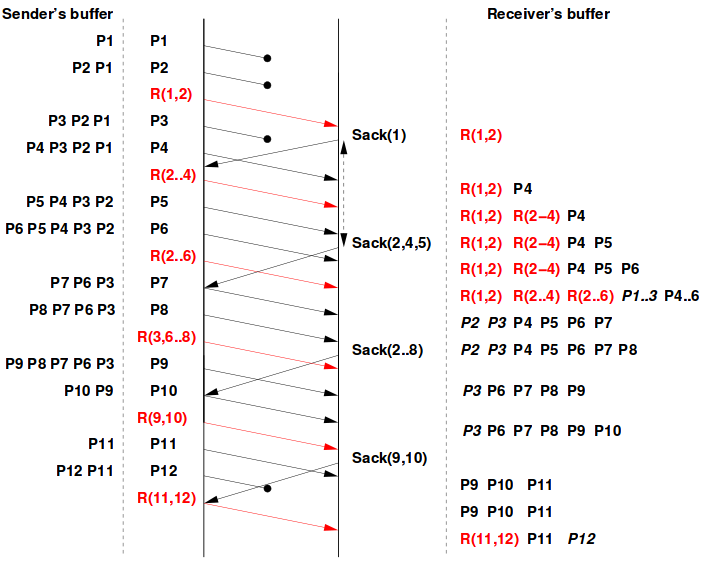
\includegraphics[scale=0.5]{img/Tetrys.png}
  \caption{Echanges de paquets avec $k=2$}
  \label{tetrys}
\end{figure}


Pour un paquet codant $n$ autres paquets, si on a perdu $m$ ($m<n$) paquet avant la réception de ce paquet de redondance, on enlève de celui-ci tous les $n-m$ paquets connus. A l'issue de la réception de $m$ paquets de redondance, la matrice de taille $m\times m$ se voit effectuée un pivot de Gauss pour retrouver les différents paquets. Le décodage sera donc bien plus efficace que du RLNC sur tous les paquets, où la matrice à décoder serait de taille $n\times n$ quel que soit le nombre de paquets perdus. 

Autant de paquets présents dans la fenêtre d'emission de l'envoyeur sont codés dans le paquet de redondance. Les paquets acquittés (de façon sélective avec SACK) sont enlevés de la fenêtre d'emission, qui est élastique, et donc du prochain paquet de redondance. Le receveur saura que l'acquittement a bien été reçu lors de la réception du paquet de redondance qui ne contiendra plus les paquets acquittés.
Tetrys est ainsi résistent aux pertes d'acquittement, et supporte l'absence totale d'acquittement aussi. Le paquet codé sera simplement une combinaison linéaire de tous les paquets précedemment envoyés.
Le taux de redondance, ainsi que la fréquence des acquittement sotn deux paramètres de Tetrys. Si la fréquence des acquittements augmente, les paquets codés seront plus simple, le décodage sera lui aussi plus simple mais le débit utile sera moins élevé. De même avec le taux de redondance.

En plus de la fiabilité totale permise par Tetrys et du délai de recouvrement de paquets perdus indépendants du RTT, il est possible de ne souhaiter qu'une fiabilité partielle, totalement adaptée au streaming vidéo par exemple. L'idée est de se contenter d'un certain pourcentage de paquets, selon l'application. Un heuristique permet d'approximer le taux de redondance minimal pour satisfaire les critères de l'application.
Une amélioration potentielle de ce framework serait le contrôle de congestion.
%on the fly
%RLNC with F256 with SACK de seen packets
%send repair each k packet.
%If n lost, need n repair. gauss on n only, known packets are taken out from the repair packets LOW DECODE


%Ack --> reduced sender's window ACK LOSS RESISTENT + elastic window

%R en parametre (à améliorer)
%Fack paramétrable (à adapter??) ++ = decode -- goodput --

%recover lost packets quite fast
%idea : if too many, maybe discard to avoid tcp timeouts ACCEPTABLE FOR STREAMING

%Si packet ok, receveier sends SACK, sender receives SACK and delete packet from window. Receiver receives repair packet without SACKed packet, and removes it from his buffer

%tetrys mieux que FEC

%no full reliability !!!
%Minimum rdundancy ratio estimatino to satisfy streaming application requirements
%adapted to streaming



\textbf{PAS FINI}

\subsection{CoMP}
multipath
uses online coding (introduced by

\section{CTCP : Coded TCP}


\subsection{TCP/NC : TCP with Network Coding}
\label{tcpnc}

\subsection{CTCP : une évolution de TCP/NC (TCP with Netowrk Coding)}
Change les ACK de TCP:

Sliding window pour le codage (difficile de décoder dans certains de pires cas)
TCP/NC pas adaptatif car constant loss rate

COuche 3.5 OSI pour le codage

\subsection{CTCP}
Mieux que TCP/NC car adaptatif (calcul du loss rate et adaptation du redundancy rate)
Si pas de pertes, CTCP fait du TCP sans codage (cool !)

fairness entre flux de même RTT (même débit), de différents RTT (ratios pareils que TCP)

Codage couche 4
Codage de blocs indépendants (taille réglable mais à limiter pour la complexité du décodage du receveur)
Pas de sliding window pour la congestio mais gestion de tokens.


reliability ok car ack de chaque packet, et de chaque bloc qui sera free une fois acké
congestion ok

Codé dans l'userspace donc pas de modifs du kernel ni des noeuds internes donc déployable facilement


\subsubsection{Principe}
de préférence, blksize = bandwidth * delay
\textsf{numbloc} blocs de \textsf{blksize} segments
\textsf{currblk}
Dans chaque paquet, send :
\begin{itemize}
\item block number
\item  seed fro pseudo-random number generator (receiver generates the coding coefficient \textbf{what?}
\item sequence number \textsf{seqno} ($seqno^{th}$ packet sent, different from TCP byte numbering)
\item paylaod (un)coded
\end{itemize}

Composition du ack
\begin{itemize}
\item smallest undecoded block \textsf{ack\_currblk} (pour que le sender free ou non ce bloc)
\item nombre de DOFs ack\_currdof reçus du bloc ack\_currblk \textbf{why?)
\item \textsf{ack\_seqno} du paquet acké}
\end{itemize}



Le sender fait la plupart du boulot, le receiver met juste quelques infos dans le ack




baisse de RTTmin / RTTcurrent donc smooth : si le réseau est bien fait et que y'a pas de perturbation mais de la congestion, RTTmax=2*RTTmin donc comportement classique de TCP donc cool.

Si lossy link, le RTT = RTTmin ( no queue) donc le nombre de tokens peut toujours augmenter (car RTT utilisé dans le decrease donc cool). Si full capacity + loss, decrease mais maintien du max throughput

\textbf{RECEIVER}

RESULTS :
TCP et CTCP coexistent
CTCP et CTCP cool : fair (tokens convergent) + max throughput
CTCP est bien si on wget des gros fichiers ( > 1Mo) car slowstart mieux dans TCP?!


CTCP miracle  !! MAIS ATTENTION TRES SENSIBLE AU RTT JITTER
CTCP pas cool si dans le réseau, une augmentation du RTT implique pas forcement de la congestion. (dépend de la couche MAC ,Wimax a du mal apparemment) genre satellite !
\cite{satellite}
\cite{ctcpmulti}
\cite{ctcp}
\cite{tcp/nc}
\cite{tcp/ncthroughput}
\cite{ncmeetstcp}
\cite{tcpmultipath}
\cite{arqfornc}
\cite{memoryanalysis}

\bibliographystyle{acm}
\bibliography{bib}
\end{document}
